\documentclass[11pts,english,letterpaper]{article}
%\usepackage{SIunits}
\usepackage[utf8]{inputenc}
\usepackage[T1]{fontenc}
\usepackage{babel} 
\usepackage{amsmath}
\usepackage{amsfonts}
\usepackage{amssymb}
\usepackage{float}
\usepackage{geometry} 
\usepackage{rotating} 
\usepackage{graphicx}
\usepackage{xspace}
\usepackage{layout}
\usepackage{mathpazo}
\usepackage{microtype}
%\usepackage{blindtext}
\usepackage{xcolor}
\usepackage{tabularx}
\usepackage{paralist}
\usepackage{setspace}
\usepackage{makeidx}
\usepackage{multirow}
\usepackage{booktabs}
\usepackage{lscape}
\usepackage{listings}
\usepackage[margin=0.5cm,font=small,labelfont=bf]{caption}

\definecolor{dkgreen}{rgb}{0,0.6,0}
\definecolor{gray}{rgb}{0.5,0.5,0.5}
\definecolor{lgray}{rgb}{0.8,0.8,0.8}
\definecolor{mauve}{rgb}{0.58,0,0.82}

\lstset{
  language=C++,
  basicstyle=\tt\small,
  xleftmargin=1cm,
  xrightmargin=1cm,
  breaklines=false,
  rulecolor=\color{black},
%  backgroundcolor=\color{lgray},
  keywordstyle=\color{blue},          % keyword style
  commentstyle=\color{dkgreen},       % comment style
  stringstyle=\color{mauve},         % string literal style
  morekeywords={TTree},
  morekeywords={->}
}

\makeindex

\usepackage[colorlinks,linktocpage]{hyperref}


\newcommand\ERR[3][]{$\left(#2 \pm #3\right) #1$}
\newcommand\ERRm[3][]{\left(#2 \pm #3\right) #1}
\newcommand\DIF[2][]{\frac{\text{d}#1}{\text{d}#2}}
\newcommand\grad[0]{{}^\circ}
\newcommand\srcfile[1]{\texttt{src/WCSim#1}}
\newcommand\volume[1]{\textsf{\textbf{#1}}}
%\floatstyle{ruled}
%\newfloat{Beispiel}{!htb}{lop}[section]
%\restylefloat{table}
\floatplacement{figure}{!htb}



\author{Johannes Hoppenau}
\title{Set up cylindrical detector geometry using \LARGE\texttt{WCSimDetectorConstruction::ConstructWC()}}



\begin{document}
\maketitle
\tableofcontents

%===========================================

\section{Overview}
The \texttt{WCSimDetectorConstruction::ConstructWC()} method returns a pointer on a logical volumes that contains a upright cylindrical detector. The function is defined in \srcfile{ConstructWC.cc}.
At the moment the detector only consist of balcksheet and PMTs. The PMTs and the blacksheet are organized in cells. This structure should make it easy to add outer detector PMTs or a steal structure behind the blacksheet. 
I tried to write the method generic and make it possible to use it for different detectors. 

\subsection{Hirarchy of Volumes}
This section describes the the volumes use to set up the detector. (figure \ref{fig:hi})
\begin{figure}
  \begin{center}
  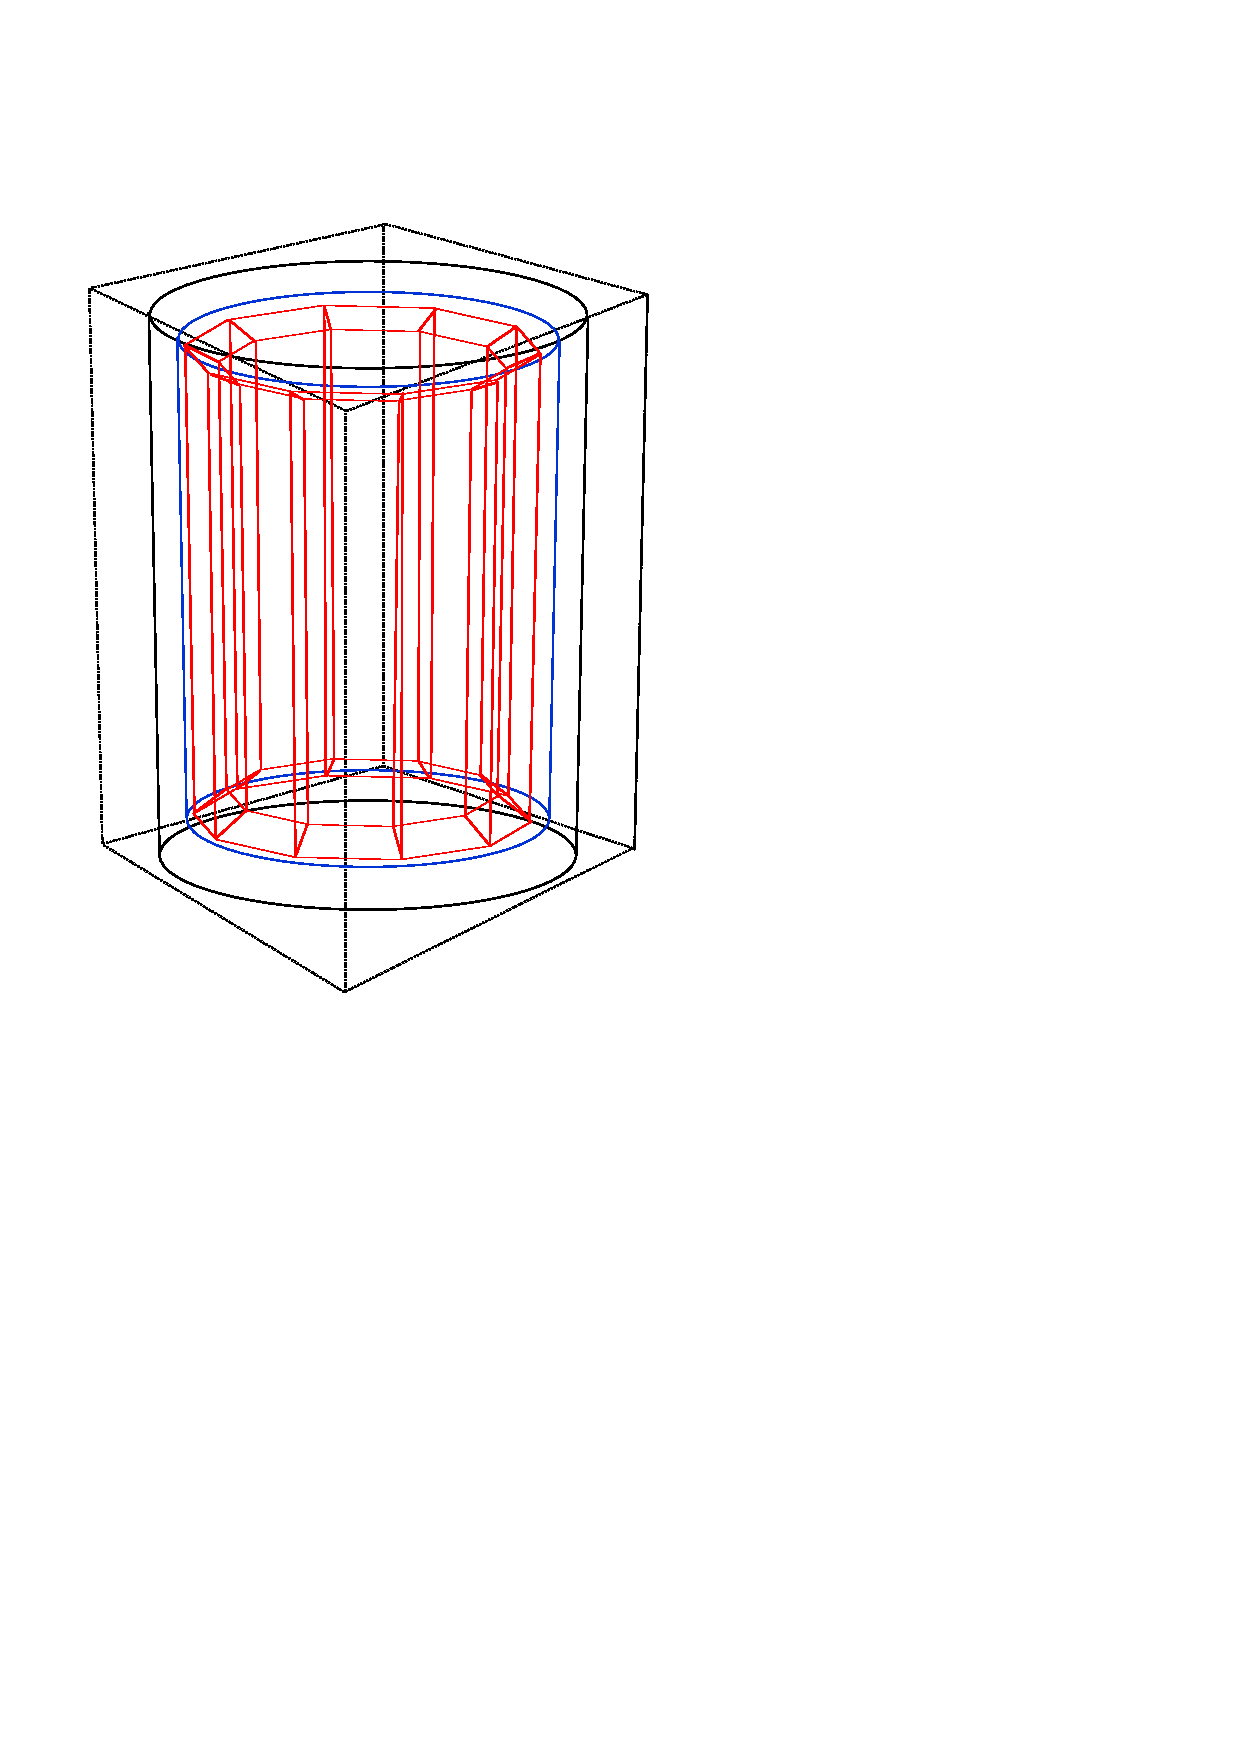
\includegraphics[width=0.45\textwidth]{expHall} 
  \hspace{0.1\textwidth}
  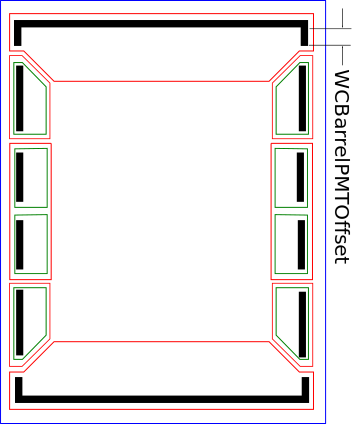
\includegraphics[width=0.35\textwidth]{annulus}
  \end{center}
  \caption{The detector geometry consists of volumes, that are placed into each other: \volume{expHall} (black dotted line) in not part of the logical volume returned by \texttt{WCSimDetectorConstruction::ConstructWC()}, \volume{WC} (black) is the volume returned by this function, \volume{WCBarrel} (blue) is filled with water, \volume{WCBarrelAnuluss}, \volume{WCBarrelBorderCell} and  \volume{WCPMTCap} (red) are the volumes the are derived into the cells (green) that hold the PMTs (not pictured) and the blacksheet (thick black line).}\label{fig:hi}
\end{figure}


\begin{description}
 \item[ExpHall] this is the world volume. It is not constructed in  \srcfile{ConstructWC.cc}
 but in \srcfile{DetectorConstruction.cc}.
 \begin{description}
  \item[WC] is a tubs filed with Air. at the moment it 
        only contains one daughter volume:
  \begin{description}
   \item[WCBarrel] is a tubs filed with water. It contains all PMTs
    (\volume{WCBarrelPMT}), blacksheet (\volume{WCBarrelCellBlackSheet}) etc.
   \begin{description}
    \item[WCBarrelAnuluss] is the main part of the detector wall. It is 
      divided into Cells, which contains the blacksheet (\volume{WCBarrelCellBlackSheet}) and one or 
      more PMTs (\volume{WCBarrelPMT}). 
      The Volume is divided in rings (\volume{WCBarellRing}) and these rings 
      are cells  (\volume{WCBarellCell}) afterward. 
    \item[WCPMTCap] This two volumes cover the bottom and the top of the 
     detector. They are not divided into cells, but contain the blacksheet
      (\volume{WCCapBlackSheet}) and PTMs
      (\volume{WCCapPMT}) directly.
    \item[WCBarrelBorder] This two Volumes connect the annuls and the caps. 
      They are divided into cells (\volume{WCBarrelBorderCell}), that contain the same number of PMTs and the same
    balcksheet as the normal annulus cells.
    
\begin{figure}
   \begin{center}
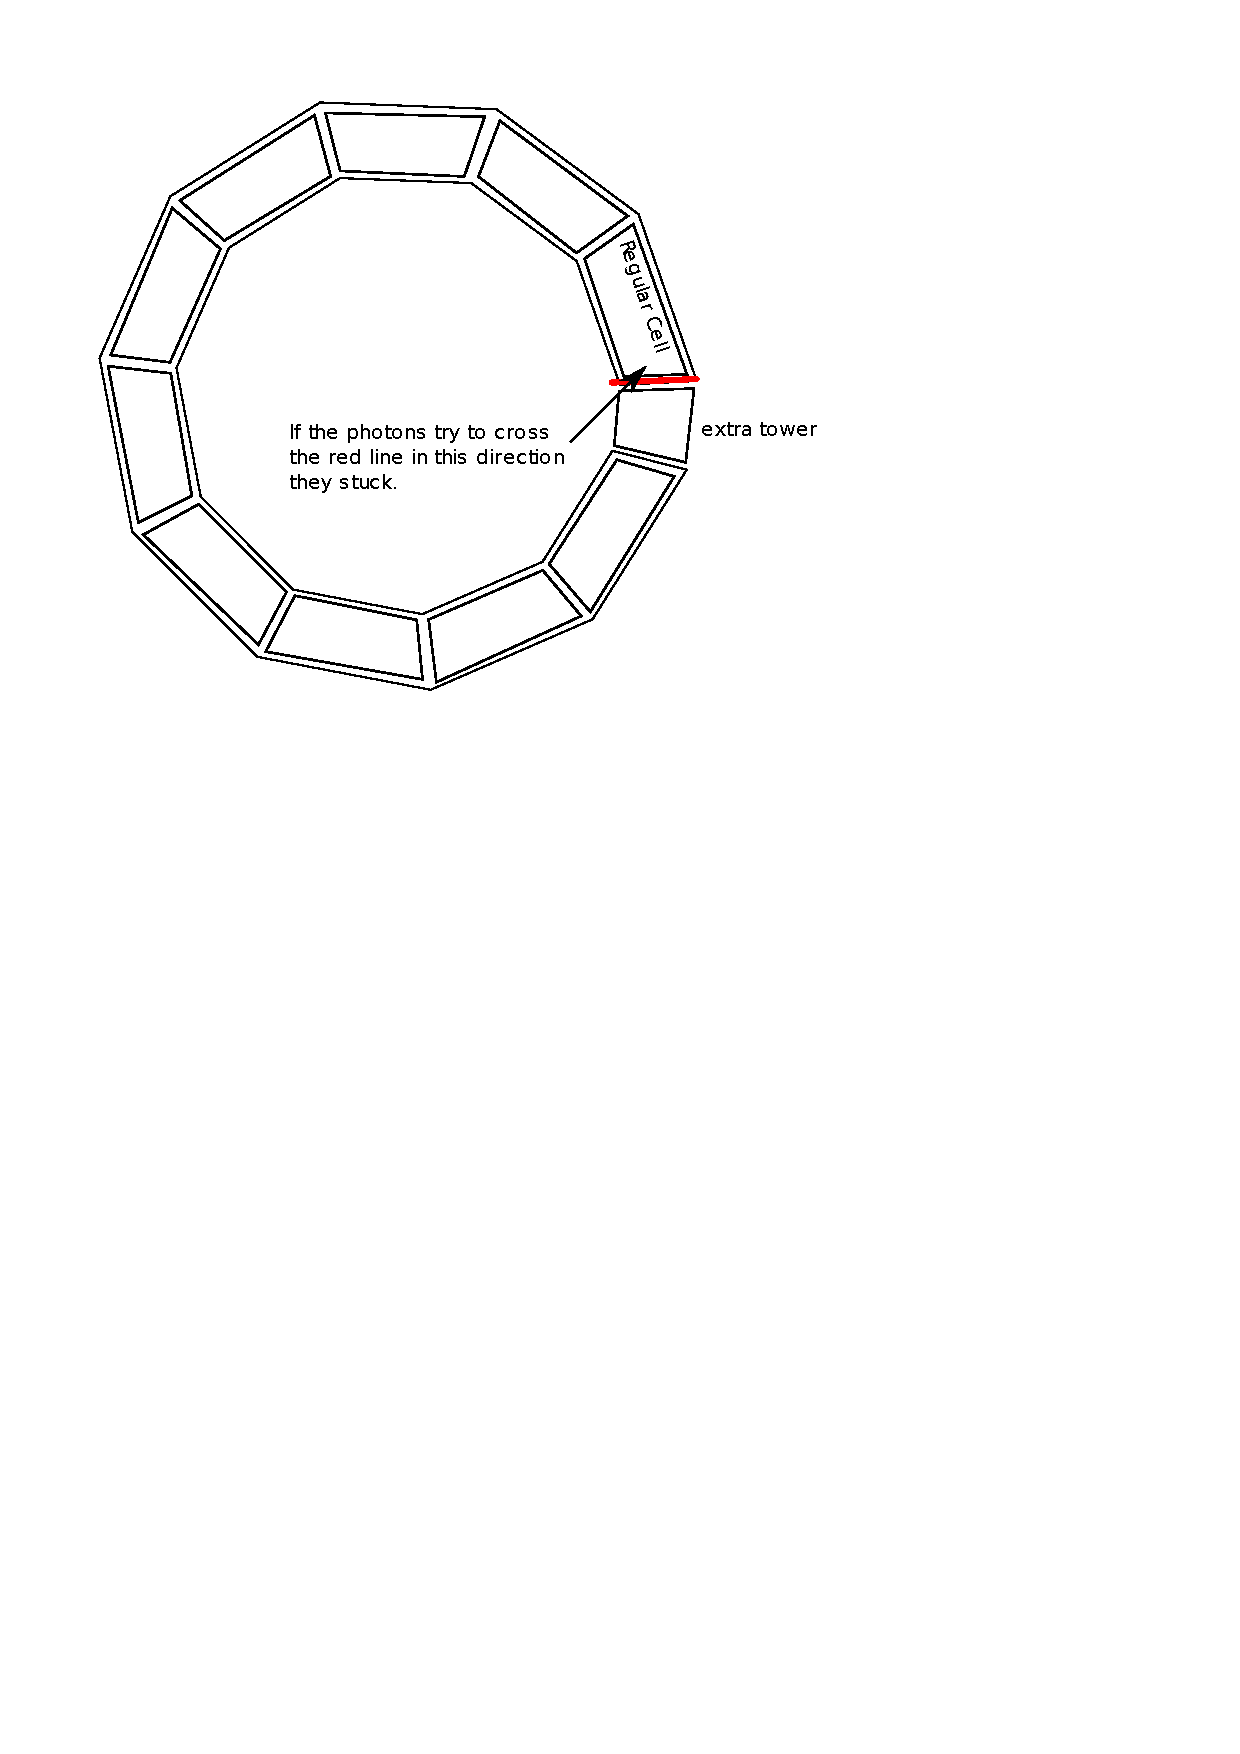
\includegraphics{extraTower} 
  \end{center}
\caption{If the number of PMTs in one cell (2) does not divides the total number of PMTs in one ring (21), there is an extra tower, that contains the remaining PMTs}\label{fig:extra}
\end{figure}

    \item[WCextraTower] is a tower that is narrower than the normal cells. It is divided 
     into cells (\volume{WCExtraTowerCell}) that contains the remaining PMTs and blacksheet (figure \ref{fig:extra}). This volume is only added if needed.
     (\volume{WCExtraTowerBlackSheet}).
    \item[WCspecialBarrelBorderCell] Also the extra tower needs special volumes to connect it 
    to the caps.
   \end{description}
  \end{description}
 \end{description}
\end{description}


%============================================

\section{Setup your own detector}

You have to store the dimensions of the detector you want to setup in member variables of  \texttt{WCSimDetectorConstruction} before calling  \texttt{WCSimDetectorConstruction::ConstructWC()}. The next section describes, which variables you have to set. The best way to to set the variables is to add an method to the \texttt{WCSimDetectorConstruction} class that set all variables. These function are at the beginning of \srcfile{ConstructWC.cc}.
You can either call this function in the constructor of \texttt{WCSimDetectorConstruction} or add it to the detector messenger (\srcfile{DetectorMessenger.cc}), if you want call it in a macro file or you want to change the detector setup dynamically. If you want to do this, you first have to use the command, that calls your function (\texttt{/WCSim/WCgeom <geometry name>}) and afterwards the detector construction command (\texttt{/WCSim/Construct}).

\subsection{Variables}
To set up a new detector geometry you have to set the following variables:

\begin{figure}
  \begin{center}
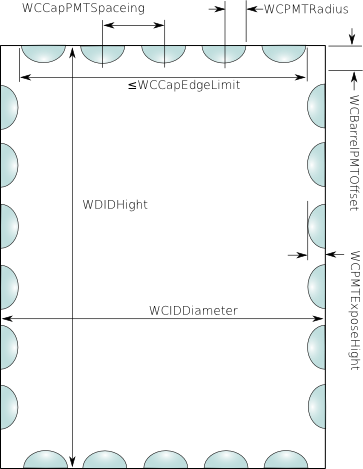
\includegraphics{variables}
  \end{center}
\caption{This are most of the variable you have to set to create a new detector geometry.}
\end{figure}


\begin{description}
\item[WCIDHeight, WCIDDiameter] This two variables are used, to setup the size of the detector. The height is the distance between the inner surfaces of the top and the bottom blacksheet and the diameter is two times the shortest distance between the inner surface of the wall blacksheet and the center of the detector.

\item[WCPMTRadius, WCPMTexposeHeight] see figure \ref{fig:pmt}. Make sure, that you only use PTMs that are known by the digitizer class. It uses the radius to identify  the PMTs. Check the beginning of \texttt{ WCSimWCDigitizer::DigitizeGate(\ldots)} in \srcfile{WCDigitizer.cc} for the supported PMTs.


\begin{figure}
  \begin{center}
    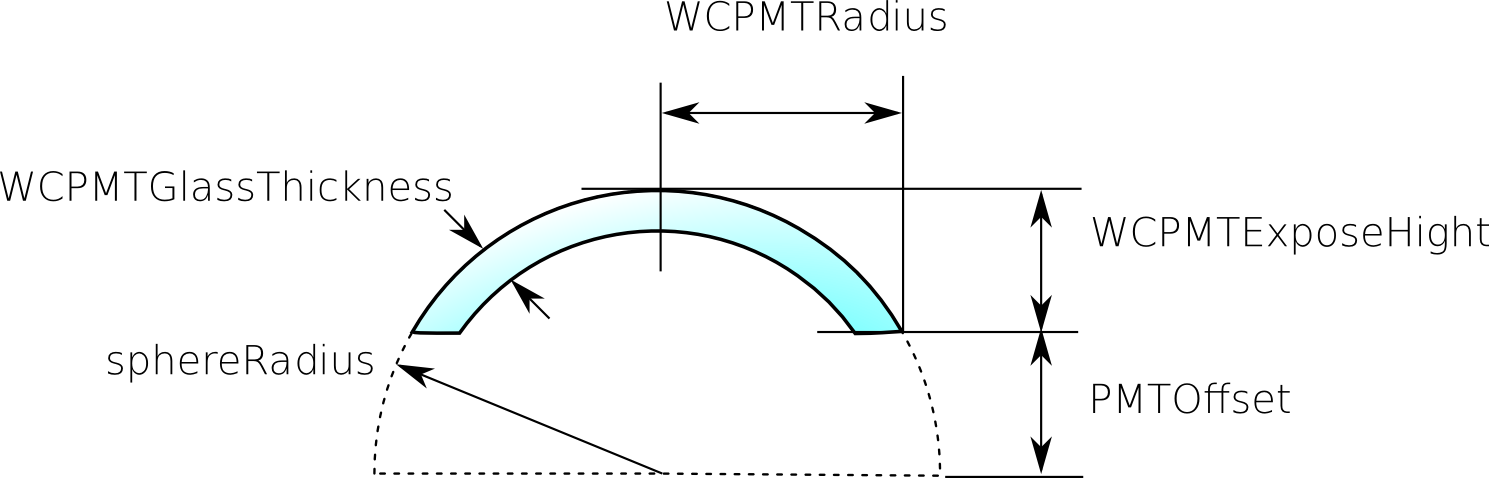
\includegraphics{PMT}
  \end{center}
\caption{The PMTs are segments of spheres. The sensitive part is the volume inside of the glass. To define the geometry of the PMTs you need to set the \texttt{WCPMTGlassThicknes}, the \texttt{WCPMTRadius}, and the \texttt{WCPMTExposeHight}}\label{fig:pmt}
\end{figure}

\item[WCPMTGlassThicknes] the thickness of the glass face.

\item[WCPMTperCellHorizontal, WCPMTperCellVertical] defines how many PMTs are there in one Cell.

\item[WCBarrelNRings] defines how many lines of PMT cells there are. 

\item[WCBarrelNumPMTHorizontal] defines the number of PMTs in one line. If WCPMTperCellHorizontal does not divide this number, there will be an extra cell in each ring, which contains the remaining PMTs.

\item[WCBarrelPMTOffset] The walls of the barrel are completely covered by PMT cells. Only a stripe at the bottom and one at the top stay free. This variable defines the width of this stripes.

\item[WCCapCellSize] defines the spacing of the PMTs at the top and the bottom of the detector

\item[WCCapEdgeLimit] This is the maximum distance between the center of the a cap and a point on a cap PMT. This length has to be smaller than half the \texttt{WCIDDiameter}. Otherwise there will be PMTs that intersect the edge of the caps.

\item[WCBlackSheetThickness] the thickness of the balcksheet.
\end {description}

All other values needed to construct set up the geometry are derived from this variables.

\subsection{Example}

\begin{verbatim}
void WCSimDetectorConstruction::SetSuperKGeometry()
{
  WCPMTRadius           =.254*m;
  WCPMTExposeHeight        =.18*m;
  WCIDDiameter          = 33.7*m;
  WCIDHeight            = 36.1*m;
  WCBarrelPMTOffset     = 0.109*m;
  WCBarrelNumPMTHorizontal  = 150;
  WCBarrelNRings        = 17.;
  WCPMTperCellHorizontal    = 4;
  WCPMTperCellVertical      = 3;
  WCCapCellSize         = 0.707*m;
  WCCapEdgeLimit        = 16.9*m;
  WCPMTGlassThickness   = .4*cm;
  WCBlackSheetThickness = 2.0*cm;
}
\end{verbatim}

This is the superK setup. This method is located at the beginning of \srcfile{ConstructWC.cc}. It is called in the constructor of \texttt{WCSimDetectorConstruction}.
In SK the PMTs are arranged in $4 \times 3$ cells (\texttt{WCPMTperCellHorizontal} and \texttt{WCPMTperCellVertical}). 
All in all there are 51 lines PMTs (3 lines in each cell times 17 lines of cells (\texttt{WCBarrelNRings})). Each line contains 150 PMTs (\texttt{WCBarrelNumPMTHorizontal}). As 150 divided by 4 is 37.5, there are 37 regular $4 \times 3$ cells and one $2 \times 3$ cell in one line.

The horizontal spacing of the PMTs is
\[
\frac{\texttt{WCIDHeight} - 2\cdot\texttt{WCBarrelPMTOffset}}
{\texttt{WCBarrelNRings} \cdot \texttt{WCPMTperCellVertical}}
= 0.703 \mathrm{m}.
\]
between the bottom (and top) blacksheet and the calls on the wall, there is a gap of 11cm (\texttt{WCBarrelPMTOffset}).

The caps are completely filled with PMTs, because \texttt{WCCapEdgeLimit} is equal to the detector diameter. 



\subsection{Warnings}
If the PMTs have a large \texttt{WCPMTExposeHeight} and there is not enough space between the PMTs and the borders of the cells, the PMTs could intersect the edge of the border cells, because the border of these cells are slanted (see figure \ref{fig:warning}). 

This can also happen at the caps if \texttt{WCCapEdgeLimit} is close to the inner radius of the detector and \texttt{WCBarrelPMTOffset} is small.

\begin{figure}
  \begin{center}
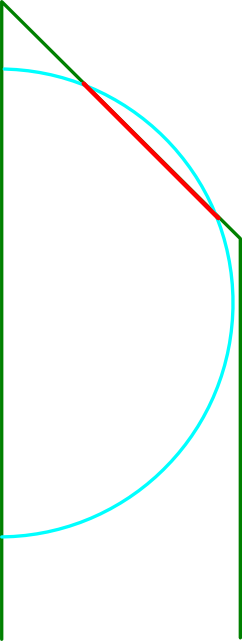
\includegraphics{warning}
  \end{center}
\caption{The topmost and bottom PMTs could  intersect the border of the cells.} \label{fig:warning}
\end{figure}

During the setup of the geometry is checked if the PMTs at the wall intersect each other or the border of the cells. You should see a lot of the flowing lines:\\
\texttt{Checking overlaps for volume WCBarrelPMT ... OK!}\\
If you see warnings instead, it is likely, that there are too large or too many PMTs.

There is no check if the placement of the PMTs on caps is correct. It would take to much time to do this check every time, because there are too many PMTs in side a single volume\footnote{It would be nice to nice to implement a check if a PMT is close to the edge of the cap and do to the test if the placement s correct only for the PMT that are close to the edge.}. 
 
 
%============================================


\section{root2zbs and superscan}
WCSim writes sores the results of a simulation in a root file. You can set the name and path of this file in the \texttt{vis.mac} file using the \texttt{/WCSimIO/RootFile} command. To view the results of the simulation with superscan, you have to convert it into a zbs-file first. To do this use \texttt{root2zbs <inpu file> <output file>}.

To open this file with superscan you need the \texttt{geofile.txt} WCSim produces and a special version of superscan, that can read in this file. In this file the positions and orientations of all PMTs and the size of the detector is store. To let superscan know, that there is a geofile, you have to set the \texttt{G4GEOFILE} environment variable to the path of this file.


\begin{figure}
  \begin{center}
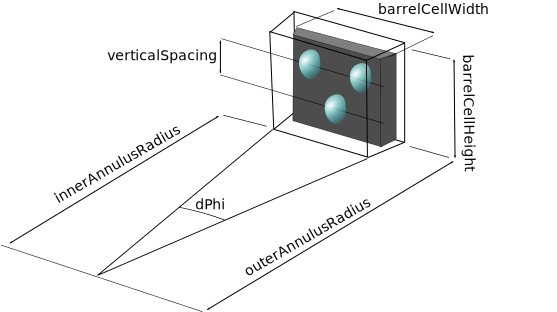
\includegraphics{Cell}
  \end{center}
\caption{Each cell holds blacksheet and multiple PMTs. All labeled length are calculated automatically. In the current version, the PMTs are distributed equally in horizontal and vertical direction.}
\end{figure}
\end{document}
